\subsection{Trajectory Optimization}
\label{sec:trajopt}

We demonstrate end-to-end differentiation through contact using an
implementation of contact-implicit iLQR with Drake~\cite{bib:kurtz2022contact}.
To compute a local feedback controller and optimal trajectory, iLQR for a system
with discrete dynamics $x_{k+1} = f(x_k, u_k)$ must compute derivatives with
respect state $\partial f/\partial x_k$ and control inputs $\partial f/\partial
u_k$. In this demonstration, the task is for the Kinova Gen3 robot arm to move a
ball on a plane from a starting position to a target position
(Fig.~\ref{fig:kinova_gen3}). We use the exact model and environment setup
described in~\cite{bib:kurtz2022contact}, with all geometries modeled with
hydroelastic contact~\cite{bib:elandt2019pressure} and a time step of 10 ms over
a 0.5 s time horizon. The method is able to efficiently solve for an optimal
trajectory involving contact between the arm and the ball without explicitly
dictating a contact sequence.

\begin{figure}[!h]
    \centering
    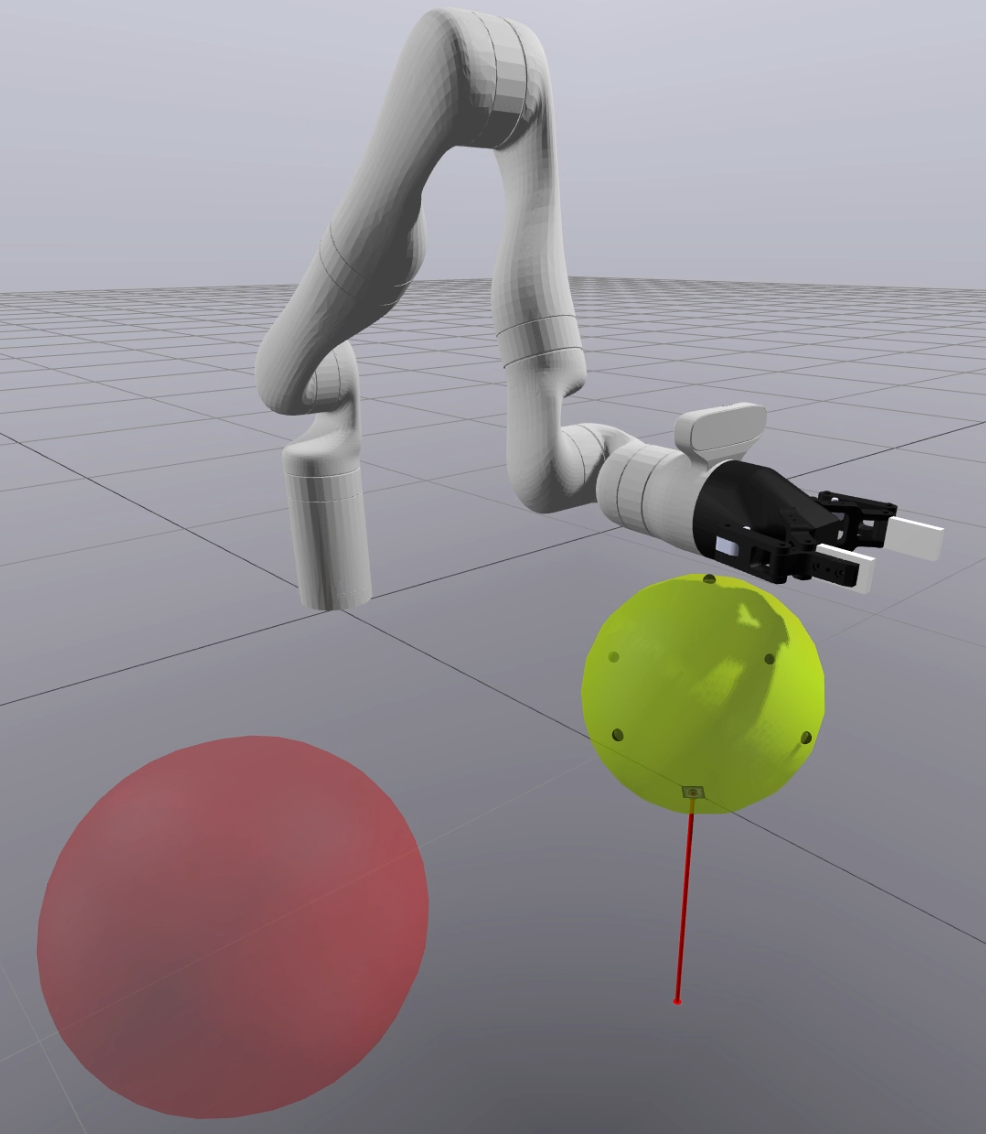
\includegraphics[width=0.49\columnwidth]{figures/TestCases/iLQR/kinova0.png}
    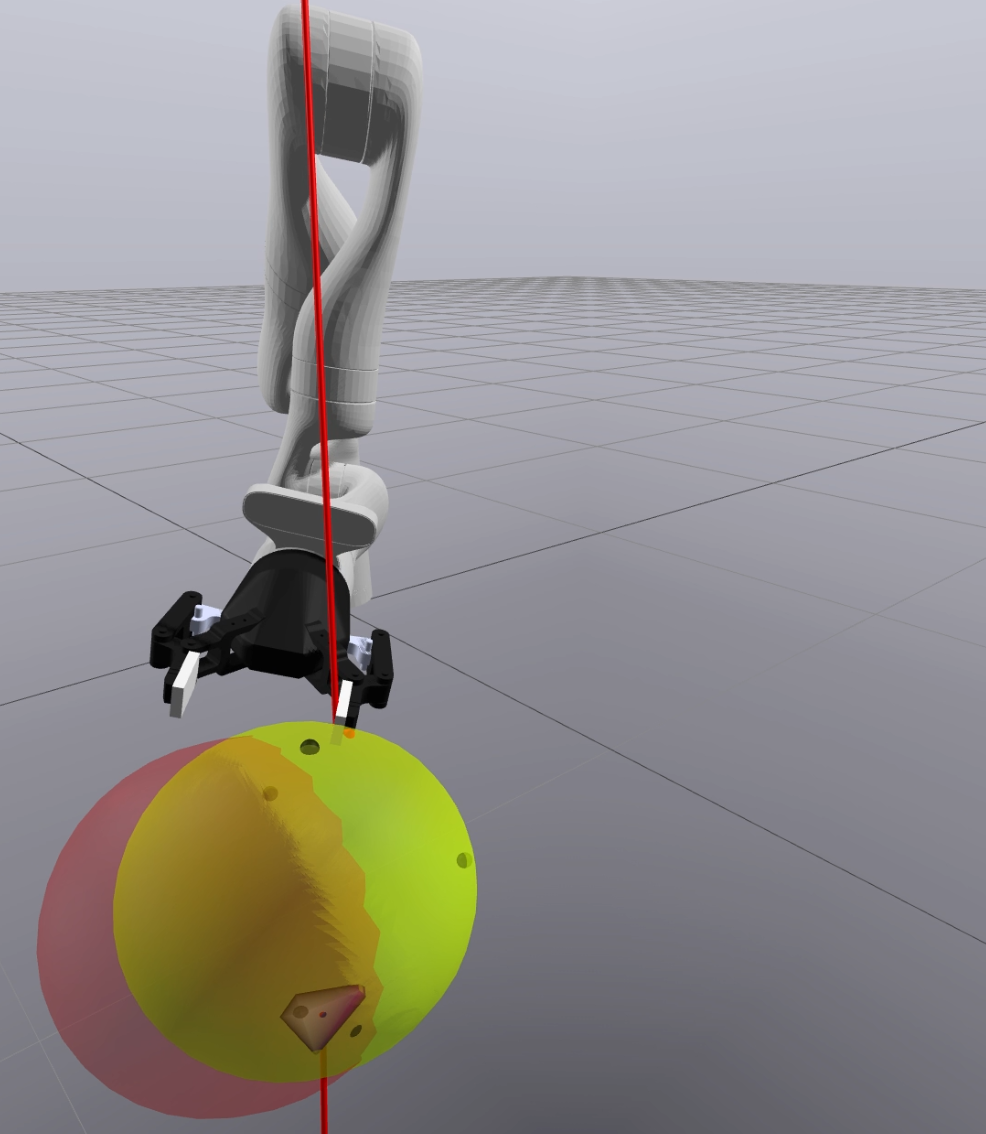
\includegraphics[width=0.49\columnwidth]{figures/TestCases/iLQR/kinova1.png}
    \caption{Keypoints of an optimal trajectory found by iLQR for the arm moving the ball to the target position (red).}
    \label{fig:kinova_gen3}
\end{figure}